%% February 2017, 

\documentclass[12pt, notes=show,handout]{beamer}
\usetheme[width=0cm]{Goettingen}
\usecolortheme{rose}
\useoutertheme{default}
\setbeamerfont{caption}{size=\scriptsize}
\setbeamertemplate{navigation symbols}{}

\addtobeamertemplate{navigation symbols}{}{%
	\usebeamerfont{footline}%
	\usebeamercolor[fg]{footline}%
	\hspace{1em}%
	$\dfrac{\insertframenumber}{\inserttotalframenumber}$
}

\usepackage{hyperref}
\usepackage{fontspec} 
\setsansfont{Futura LT}


\usepackage{arydshln}
\usepackage{amsmath}

\usepackage{mathptmx}
\usepackage{latexsym}
\usepackage{mathtools}
\usepackage{multirow}
\usepackage{caption}



\title{
	JIPI 2017:\\
	Culture changes \& Economic Equilibrium.
}

\institute{9 Febrer}

\author{Simon Carrignon}

\date{
	\scriptsize
	\begin{columns}
		\begin{column}{.3\textwidth}
			\begin{center}
				Barcelona Supercomputing Center	\\
				
\includegraphics[height=1cm]{images/bscLogo.jpg} \hspace{2cm}
			\end{center}
		\end{column}
		\begin{column}{.3\textwidth}
			\begin{center}
				Univ. Pompeu Fabra Complex System Lab.\\
				\includegraphics[height=1cm]{images/upfLogo.jpeg} %declare logo image with an alias here 
			\end{center}
		\end{column}
	\end{columns}

}
\begin{document}
\begin{frame}
	\maketitle

\end{frame}

\section{Introduction}

\begin{frame}{Cultural Evolution}
    Social Traits:
    \begin{center}
	\begin{table}
	    \center
	    \begin{tabular}{ccc}
		\uncover<2->{\includegraphics[height=3cm]{images/m80}} &
		\uncover<3->{\includegraphics[height=3cm]{images/m90}} &
		\uncover<4->{\includegraphics[height=3cm]{images/m10}} \\
		\uncover<2->{80's} & \uncover<3->{90's} & \uncover<4->{now}
	    \end{tabular}
	\end{table}
    \end{center}
    \uncover<5->{How they Evolve?}\uncover<6>{ Cultural Evolution }
\end{frame}


\begin{frame}{Cultural Evolution}
    \begin{itemize}
	\item<5->{ culturally transmitted, socially learnt}
	\item<6->{ similar patterns}
    \end{itemize}
	\begin{center}
		\uncover<4->{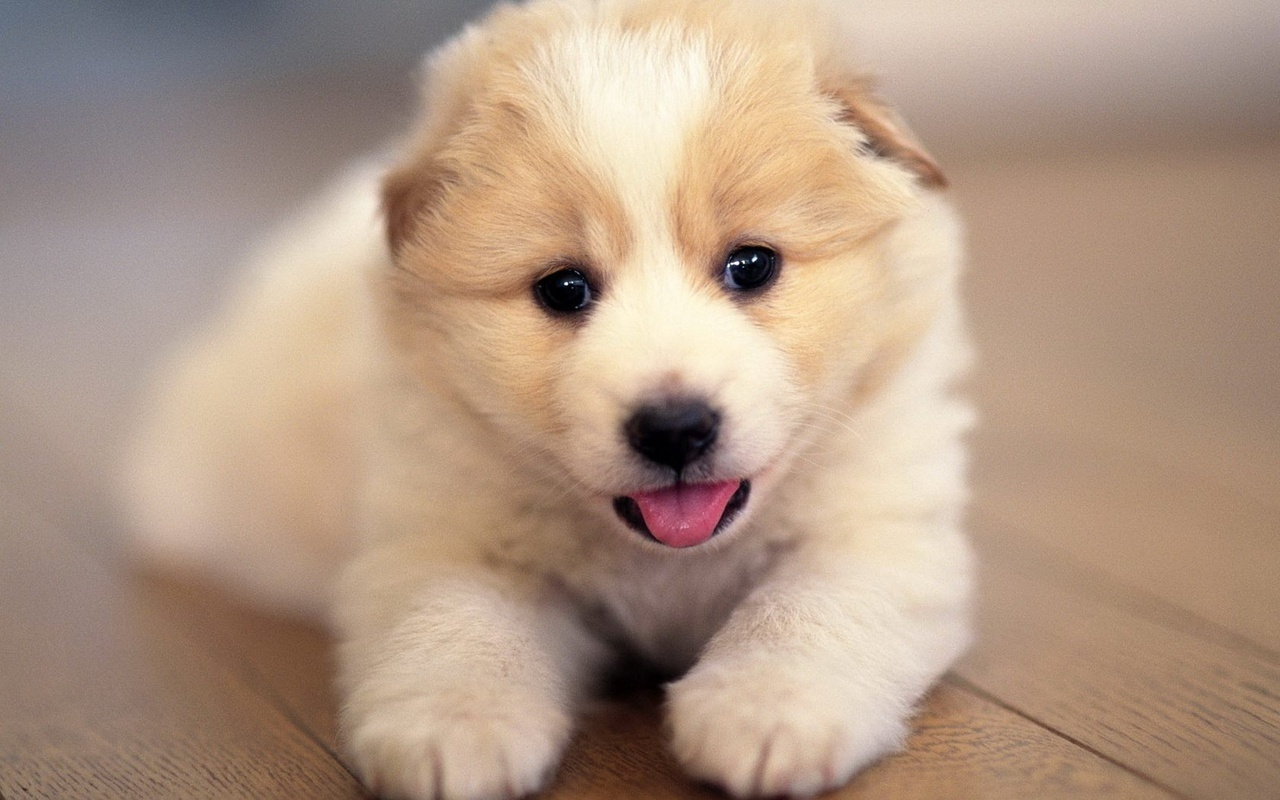
\includegraphics[width=3cm]{images/cutdog}}\\
		\vspace{.5cm}
		\uncover<2->{\includegraphics[width=2.5cm]{images/cutbaby}}
	    \hspace{1cm}
	    \uncover<3->{ \includegraphics[width=2cm]{images/pottery}}
	\end{center}
    \uncover<7>{$\rightarrow$ What mechanism drive the evolution of such traits?\\
    \invisible<1->{$\rightarrow$ What mechanism }generate such pattern?}
\end{frame}

\begin{frame}{What Generate Those Cultural changes?}
	Simple mechanisms (Bentley et al, 2004):
	\begin{itemize}
		\item<2->Random Copy 
		\item<3-> Frequency biased (conformist/anti-conformist\dots)
		\item<4->\dots	
	\end{itemize}
	\uncover<2>{\begin{figure}
		\begin{columns}
			\begin{column}{.8\textwidth}
				\centering
				\includegraphics[width=.6\textwidth]{images/powerlawrepartition.jpg}
			\end{column}
			\begin{column}{.3\textwidth}
				\tiny
				Square: male names\\
				Circle: female names\\
				Dotted and plain lines: model result with different copy probabilities.\\
			From Bentley et al,~2004.
			\end{column}
		\end{columns}
	    \end{figure}}
\end{frame}

\section{Economic Traits}


\begin{frame}
	\begin{center}
	    What if such mechanisms act on traits linked to economics?
	\end{center}
\end{frame}

\begin{frame}
	\begin{center}
	    \only<1>{\includegraphics[width=.8\textwidth]{images/boubou1.png}}
	    \only<2>{\includegraphics[width=.8\textwidth]{images/boubou2.png}}
	    \only<3>{\includegraphics[width=.8\textwidth]{images/boubou3.png}}
	\end{center}
\end{frame}
\begin{frame}{Co-evolution of Economy and Culture}

%How Simple Cultural Dynamics influence Economy That in turn will influence cultural dynamics.
    \vspace{2cm}
    \begin{center}
	\begin{overlayarea}{\textwidth}{\textheight}
	    \only<1>{\includegraphics[width=\textwidth]{images/map1.png}}
	    \only<2>{\includegraphics[width=\textwidth]{images/map2.png}}
	    \only<3>{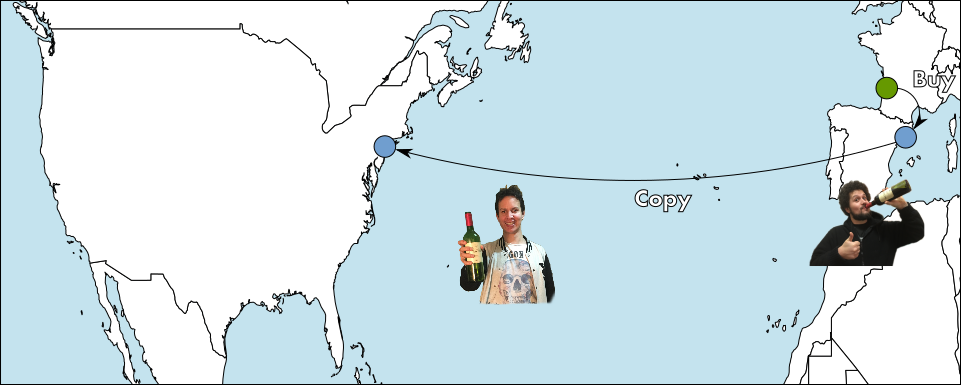
\includegraphics[width=\textwidth]{images/map3.png}}
	    \only<4>{\includegraphics[width=\textwidth]{images/map4.png}}
	    \only<5>{\includegraphics[width=\textwidth]{images/map5.png}}
	    \only<6>{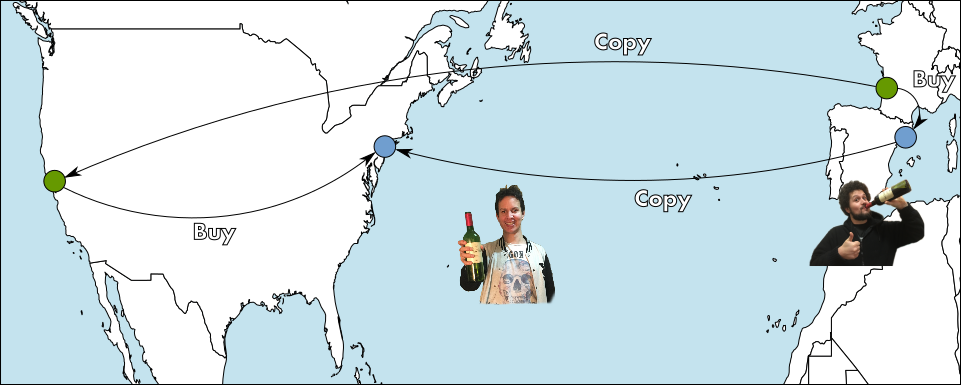
\includegraphics[width=\textwidth]{images/map6.png}}
	    \only<7>{\includegraphics[width=\textwidth]{images/map7.png}}
	    \only<8>{\includegraphics[width=\textwidth]{images/map8.png}}
	    \only<9>{\includegraphics[width=\textwidth]{images/map9.png}}
	    \only<10>{\includegraphics[width=\textwidth]{images/map10.png}}
	    \only<11>{\includegraphics[width=\textwidth]{images/graph1.png}}
	    \only<12>{\includegraphics[width=\textwidth]{images/graph2.png}}
	    \only<13>{\includegraphics[width=\textwidth]{images/graph3.png}}
	\end{overlayarea}

    \end{center}
\end{frame}

\begin{frame}{Co-evolution of Economy and Culture}

%How Simple Cultural Dynamics influence Economy That in turn will influence cultural dynamics.
    \begin{center}
	\includegraphics[width=\textwidth]{images/cooev.png}	
    \end{center}

\end{frame}

\section{ABM Framework}


\begin{frame}{A General Agent Based Framework }

    Computer Model
    \begin{center}
	\includegraphics[width=.8\textwidth]{images/cooev.png}	
    \end{center}
\end{frame}

\begin{frame}{Why Computer Model?}
    \vfill
    Understand general dynamics and properties of such systems:
    \vfill
	\begin{itemize}
	\item Different Cultural Mechanisms
    \vfill
	\item Different Trade Assumption
    \vfill
	\item Network Constraints
    \vfill
	\item \dots
    \vfill
	\end{itemize}
    {\large Study Cultural evolution \textbf{is not} possible without archaeology studies}
    \vspace{.5cm}
    \uncover<2->{
    \begin{center}
	and
    \end{center}
    \vspace{.5cm}
}

\uncover<3>{    {\large Simulation as a tool to implement and test hypothesis made on Historical questions.}\\
    \vspace{.5cm}
	{\scriptsize(Carrignon et al., Model \& Simluation 7, May 2016, BCN)}
    }
	
\end{frame}
	

\begin{frame}{Results: Economic Dynamic}
    \begin{figure}[!h]
	\centering
	\begin{tabular}{ c c}
	    Neutral Model & Trading Model \\
	    \includegraphics[width=5cm]{images/ScoreEvolutionForRandom-G3N500.pdf}
	    & 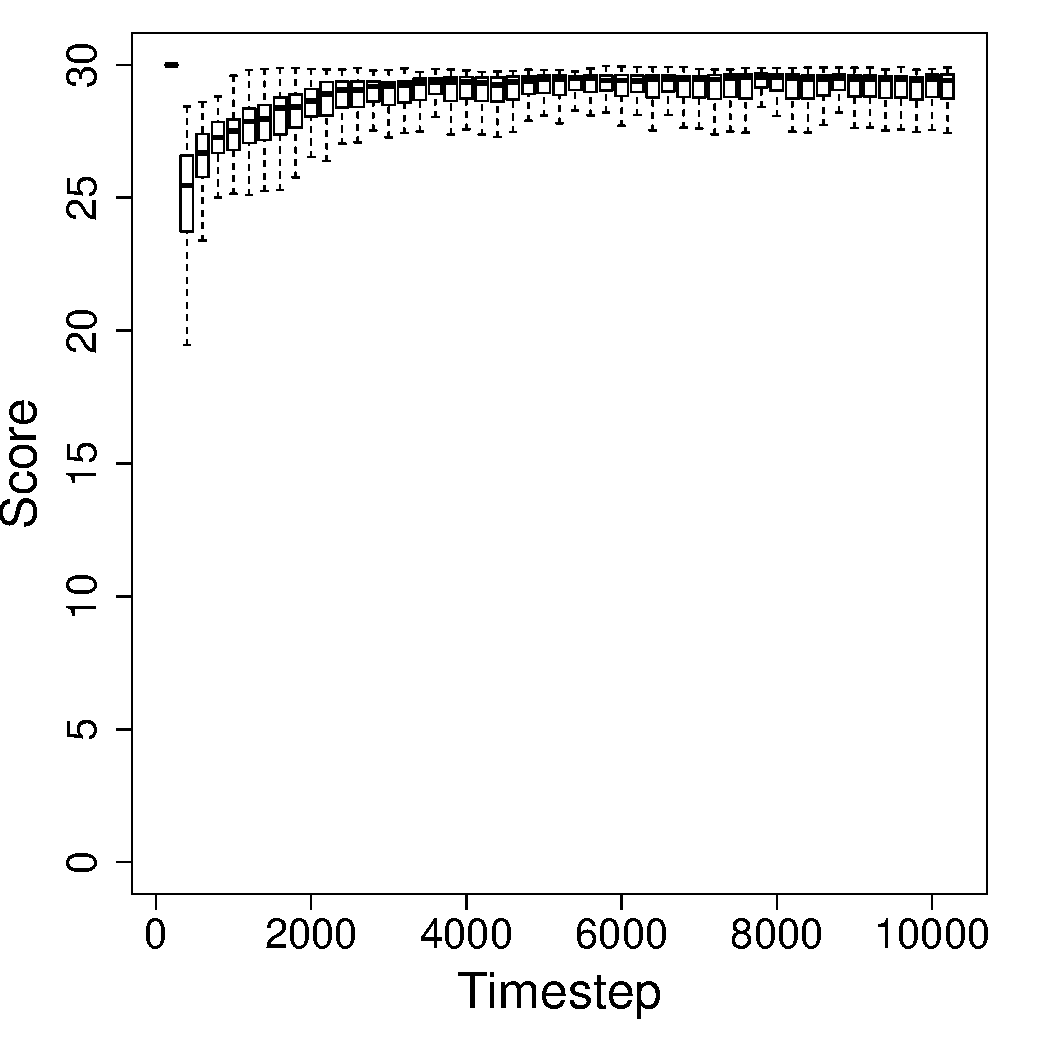
\includegraphics[width=5cm]{images/ScoreEvolutionForTrade-G3N500.pdf}

	\end{tabular}
	\caption{Evolution of the score within the two different models for two typical run with 500 agents and 3 goods evolving during 10000 timestep.}%%
	\label{fig:scoreEvol}
    \end{figure}
\end{frame}
    


\begin{frame}{Results: Economic Dynamics}
	\begin{figure}
	    \caption{Example for 3 goods and 500 agents}
	    \begin{columns}
		\column{.5\textwidth}
		\includegraphics[height=\textwidth]{images/ClearingPriceDistanceEvolutionForTrade-G3N500.pdf}\\
	    \end{columns}
		@~Equilibrium: personal values  $\rightarrow$ optimal (shared) values.
	\end{figure}
	
\end{frame}

\begin{frame}
	\begin{center}
		\Large
    Thank for you attention!\\
%		What was the nature of Roman economy?\\
		\includegraphics[width=2cm]{images/LOGO-ERC.jpg} \hfil	\includegraphics[width=3cm]{images/epnetLogo.png}\\
		\vspace{1cm}
		\scriptsize
			http://www.roman-ep.net/\\
			@epnetproject\\
			fb.com/EPNetProject\\
			@simoncarrignon
	\end{center}


\end{frame}

%\begin{frame}
%    \Huge
%    Thank for you attention!
%\end{frame}
\end{document}


